%\setcounter{chapter}{5}
\chapter{Normalization verification}
\label{Sect:norm}
\counterwithin{equation}{chapter}

To prove the correct normalization of the obtained results, one is used to carry out the comparison with previously existing data (if they are available in the desired kinematic region) or some theoretical calculations/parametrizations. In the latter case, one usually is focused on some well-understood quantities such as the elastic cross section. The elastic cross section is almost perfectly known and parametrized for the reactions off a free proton. Meanwhile, the quasi-elastic cross section for the scattering off nucleons in a nucleus is less understood and somehow lacking the same quality of theoretical description. However, several techniques have been developed on this matter, and the attempt to use them to prove the normalization of the results of this analysis was made. The details are given in this Chapter.


\subsection*{ Peter Bosted parametrization}

The set of Bosted parametrizations of inclusive cross sections off different targets~\cite{Bosted_fit,Bosted:2007xd} includes the modeling of the quasi-elastic cross section off various nuclei (including the deuteron). This modeling is based on the method of the quasi-elastic cross section estimation that was developed in the framework of the Relativistic Fermi Gas model and described in Refs.~\cite{Amaro:2004bs,Alberico:1988bv,Donnelly:1998xg}. The general idea of this method is sketched below. 

The differential cross section for the quasi-elastic scattering of a nucleus can be calculated in the laboratory frame as
\begin{equation}
\frac{d\sigma}{d\Omega dE'} = F^{QE}\left [ \frac{d\sigma}{d\Omega} \right ]_{Mott}\left (v_{L}G_{L}^{QE} + v_{T}G_{T}^{QE} \right ),
\end{equation}
where \vspace{-1em}
\begin{itemize}
\item the quantity in the square brackets is the Mott cross section of the electron scattering off a point-like charge that is defined as
\begin{equation}
\left [ \frac{d\sigma}{d\Omega} \right ]_{Mott} = \left [ \frac{2\alpha E'}{Q^{2}}\cos \frac{\theta_{e'}}{2} \right ]^{2},
\label{eq:mott}
\end{equation}
with $E'$ and $\theta_{e'}$ being the energy and the polar angle of the scattered electron in the Lab frame, $Q^{2}$ the photon virtuality, and $\alpha=1/137$ is the fine structure constant;   \vspace{-0.5em}
\item the functions $G_{L}^{QE}$ and $G_{T}^{QE}$ are defined as
\begin{equation}
\begin{aligned}
&G_{L}^{QE}&=~&\frac{\kappa}{2\tau}\left ( ZG_{E_{p}}^{2}+NG_{E_{n}}^{2} \right )~~\textrm{and}\\
&G_{T}^{QE}&=~&\frac{\tau}{\kappa}\left ( ZG_{M_{p}}^{2}+NG_{M_{n}}^{2} \right ),
\label{eq:eee}
\end{aligned}
\end{equation}
where $\tau = \frac{|Q^{2}|}{4m_{N}^{2}}$ and $\kappa = \frac{q}{2m_{N}}$ with the photon momentum magnitude $q$ and the nucleon mass $m_{N}$. Also $Z$ and $N$ are the numbers of protons and neutrons in the nucleus, respectively, and $G_{E}$ and $G_{M}$ are so-called Sachs electric and magnetic form factors that are related to the charge and magnetization density of the corresponding nucleon, respectively;  \vspace{-0.25em}
\item  $v_{L} = \left [\frac{\tau}{\kappa^{2}} \right ]^{2} $ and $v_{T} = \frac{\tau}{2\kappa_{2}} +\tan^{2}{\frac{\theta_{e'}}{2}}$ are the kinematic factors;\vspace{-0.25em} 
\item $F^{QE}$ is the nuclear scaling function.\vspace{-0.25em}
\end{itemize}

In the Bosted parametrization~\cite{Bosted_fit,Bosted:2007xd} the Sachs form factors are calculated according to Ref.~\cite{Bosted:1994tm}, which provides an empirical fit to the world data for the proton elastic electromagnetic form factors in the range 0 GeV$^{2}$$< Q^{2} <$ 30 GeV$^{2}$ and to the neutron electromagnetic form factors in the range 0 GeV$^{2}$$< Q^{2} <$ 10 GeV$^{2}$. It is noteworthy that, according to Refs.~\cite{Fed_an_note:2017,Fed_paper_2018}, the Bosted parametrization of the free proton elastic cross section (based on the same fit of proton form factors~\cite{Bosted:1994tm}) matches the measured cross section within $\sim$ 3\% in the kinematic region investigated in this analysis.

For the case of scattering of a deuterium nucleus the Bosted parametrization~\cite{Bosted_fit,Bosted:2007xd} offers two options for estimation of the nuclear scaling function $F^{QE}$ (with the first one treated as preferential), i.e.\vspace{-0.25em}

\begin{itemize}
\item using a PWIA calculation and the Paris deuteron wave function~\cite{Bosted:2007xd} or\vspace{-0.25em}

\item using the following parametrization of the scaling function taken from Ref.~\cite{Bodek:2014pka}.\vspace{-0.25em}

\begin{equation}
F^{QE}(\psi') = \frac{1.5576}{K_{F}[1 + 1.77202(\psi' + 0.3014)^{2}](1 + e^{-2.4291\psi'})}\label{eq:fqe_scaling}
\end{equation}

Here $\psi'$ is the scaling variable defined in Refs.~\cite{Bodek:2014pka,Amaro:2004bs} and $K_{F}$ is the nucleus Fermi momentum, which in the Bosted parametrization is equal to 0.0085~GeV for the deuteron.\vspace{-0.25em}

\end{itemize}


\subsection*{Approximations of the peak cross section value}

The first consistent description of inelastic electron-deuteron scattering, which in contrast to earlier calculations took into account all important contributions to the electron-nucleon interaction as well as to the final state interactions between the outgoing nucleons, was Durand's relativistic theory~\cite{Durand:1959zz,Durand:1961zz}. In 1961 in Ref.~\cite{Durand:1961zz} Durand gave a simple approximation formula for the cross section at the quasi-elastic peak, which then was being widely used by experimentalists. This formula, which is supposed to give a reasonable result for photon virtualities $<2$~GeV$^{2}$, is given by
\begin{equation}
\left [ \frac{d\sigma}{d\Omega dE'} \right ]_{peak} = \left [ \frac{d\sigma}{d\Omega} \right ]_{Mott} ( 4.57\cdot 10^{-3}) \frac{m_{N}^{2}}{pE} \left (G_{E_{p}}^{2} + G_{E_{n}}^{2} + \frac{\tau}{\epsilon}(G_{M_{p}}^{2} + G_{M_{n}}^{2})  \right )\frac{1}{1+\tau},\label{eq:durand}
\end{equation}
where $\epsilon = \left (1 +2\tau(1+\tau)\tan^{2}\frac{\theta_{e'}}{2} \right )^{-1}$, $p = q/2$ with the photon momentum magnitude $q$, $E=\sqrt{p^{2} + m_{N}^{2}}$, and all other quantities defined as above. The numerical coefficient~is~in~GeV$^{-1}$.

Since Durand's theory a lot of papers on inelastic electron-deuteron scattering~\cite{Kocevar:1967,Budnitz:1969dt,Hanson:1973vf} have tried to modify it with respect to one or the other point to get a still better understanding of the existing experimental data. Among them the most interesting is the study~\cite{Kocevar:1967}, which estimates some higher order contributions that stem from the use of complete relativistic kinematics and provides the exact formula for the peak cross section (see Eq.~(50) in Ref.~\cite{Kocevar:1967}). The result given by this formula agrees well with Durand's approximation for low $Q^{2}\sim$0.25-0.5~GeV$^{2}$ and the difference increases as $Q^{2}$ grows.



%investigates the influence of the deuteron model on the theoretical cross section and estimates some higher order contributions which stem from the use of complete relativistic kinematics. This study provides the exact formula for the peak cross section (see Eq.~(50) in Ref.~\cite{}), which for small values of $Q^{2}$ (from 0.1 to 0.15 ~GeV$^{2}$) gives the result that is in agreement with Durand's result within a percent. However, the difference between the cross section values given by these two formulae increases as $Q^{2}$ grows.

\subsection*{Checking the parametrization with previously available data}
\label{sect:prev_data}

Before applying the parametrization~\cite{Bosted_fit,Bosted:2007xd} to this particular analysis, it was firstly tested on two sets of existing data, i.e. the first set consists of six measurements obtained for beam energies from 0.5 to 1.6~GeV and $Q^{2}$ from 0.25 to 1.8~GeV$^2$~\cite{Hanson:1973vf}, while the second set includes two measurements obtained for beam energies of 9.8 and 12.6~GeV and $Q^{2}$ of 2.5 and 4~GeV$^2$, respectively~\cite{Rock:1991jy,Rock_SLAC}. The former set is especially important, since its $Q^{2}$ coverage overlaps with that of this analysis. The latter set is used as a complimentary one.

Figure~\ref{fig:hanson_QE} shows the quasi-elastic peak for the first set of measurements~\cite{Hanson:1973vf} (black points) compared with the Bosted parametrization shown as histograms. The blue histograms correspond to the case, when $F^{QE}$ was calculated by using the Paris wave function (preferential option for the deuteron target), while the green histograms correspond to $F^{QE}$ given by Eq.~\eqref{eq:fqe_scaling}. As is seen from Fig.~\ref{fig:hanson_QE}, although describing rather nicely the left and right distribution slopes, the blue histograms systematically overestimate the peak value. Meanwhile, the green histograms have worse description of the left slope and have a tendency to underestimate the peak cross sections. The parametrization histograms were produced together with the inclusive part of the spectrum to facilitate visual comparison with the experimental measurements. The green horizontal lines in Fig.~\ref{fig:hanson_QE} correspond to Durand's approximation of the peak value given by Eq.~\eqref{eq:durand}, while the red lines correspond to the predictions of the formula from Ref.~\cite{Kocevar:1967}. As is seen, the former describes nicely the experimental peak value, while the latter matches surprisingly well the maximum of the blue histogram of the Bosted parametrization.

\begin{figure}[htp]
\begin{center}
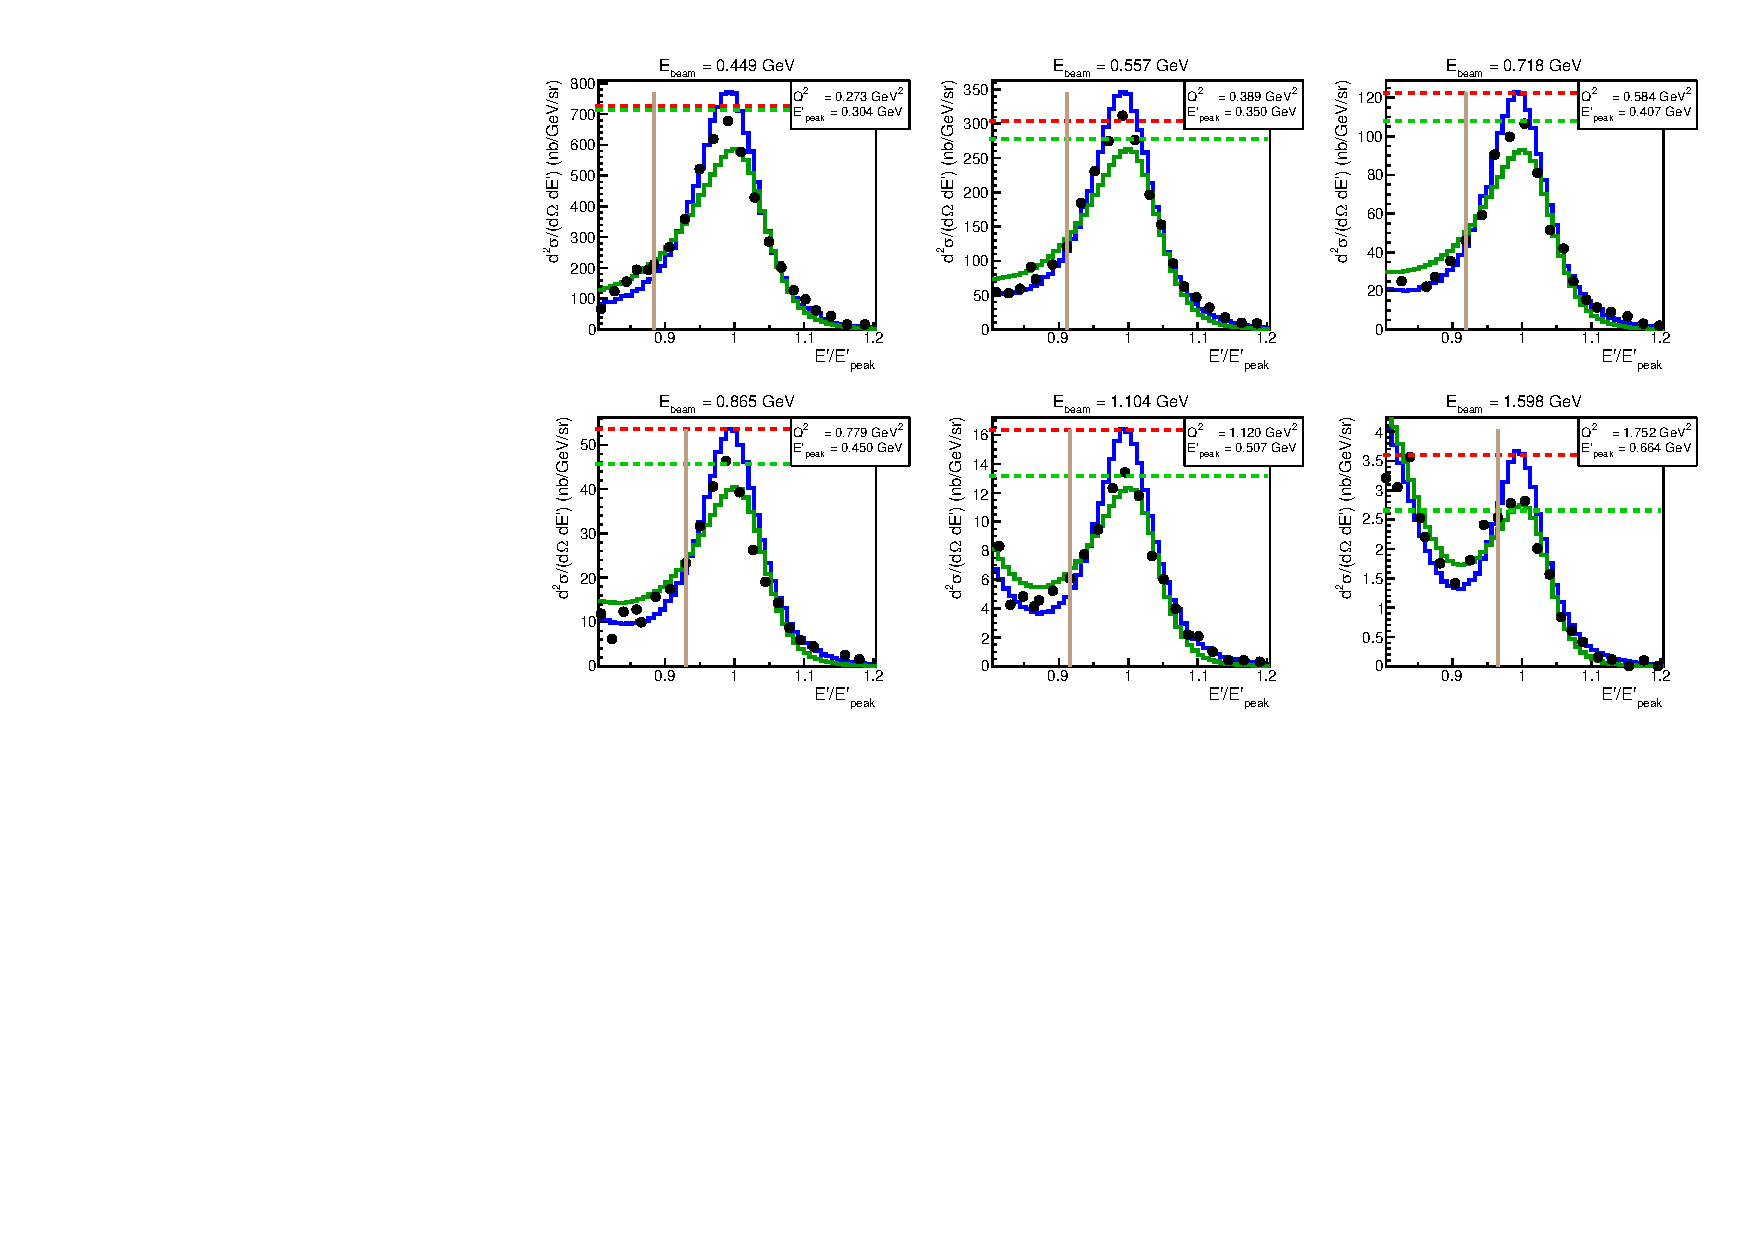
\includegraphics[width=15cm]{pictures/normalization/hanson.pdf}
\caption{\small  Data from Ref.~\cite{Hanson:1973vf} (black points) are compared with the Bosted parametrization~\cite{Bosted_fit,Bosted:2007xd} (histograms). The data uncertainties (which are on a level of 5\%) are not shown, see Ref.~\cite{Hanson:1973vf} on this matter. The blue histograms correspond to $F^{QE}$ being calculated by using the Paris wave function, while the green ones correspond to $F^{QE}$ given by Eq.~\eqref{eq:fqe_scaling}. The green horizontal lines correspond to Durand's approximation of the peak value given by Eq.~\eqref{eq:durand}, while the red lines correspond to the prediction of the formula from Ref.~\cite{Kocevar:1967}. The vertical lines correspond to the left integration limits.} \label{fig:hanson_QE}
\end{center}
\end{figure}

%\multicolumn{1}{|c|}{$\theta_{e'}$ (deg)}



\afterpage{\clearpage}
\begin{figure}[htp]
\begin{center}
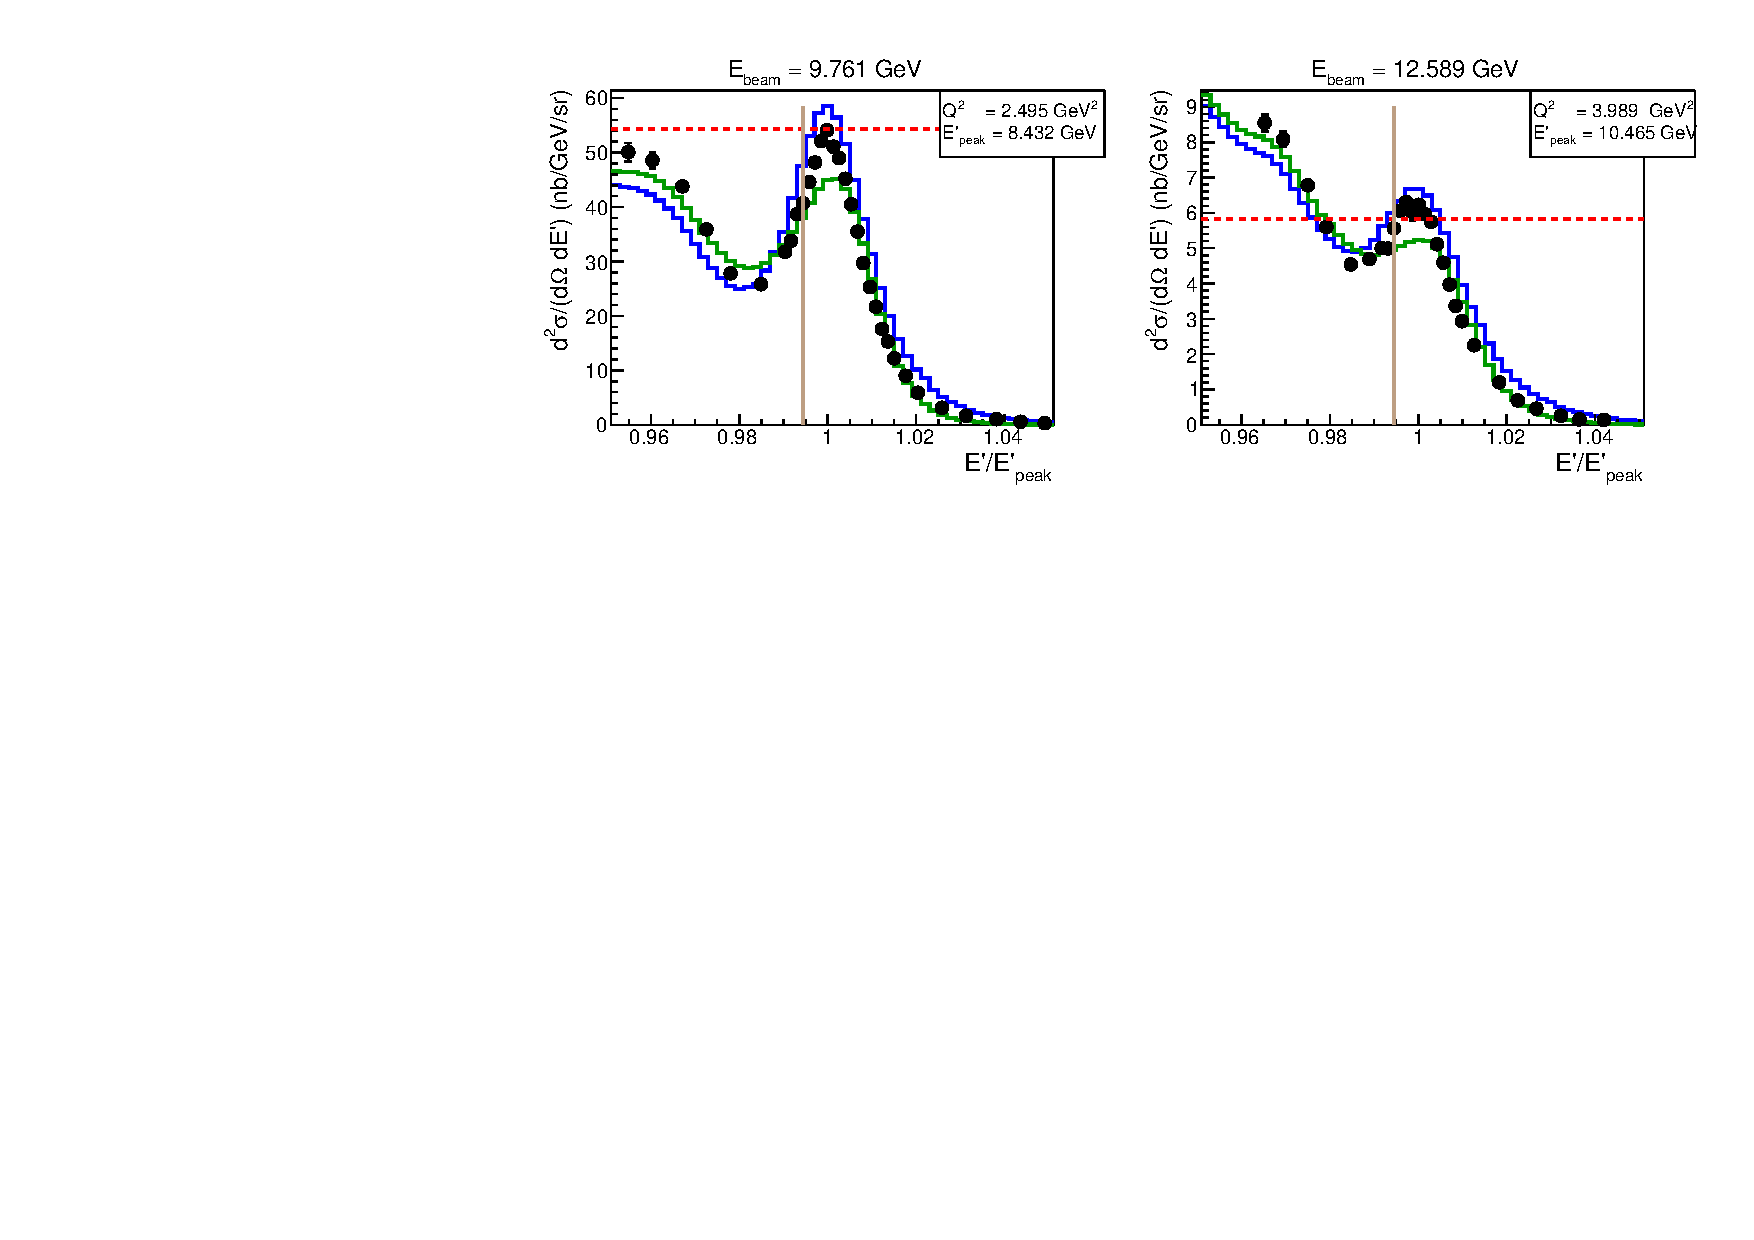
\includegraphics[width=14cm]{pictures/normalization/rock.pdf}
\caption{\small Data from Refs.~\cite{Rock:1991jy,Rock_SLAC} (black points) are compared with the Bosted parametrization~\cite{Bosted_fit,Bosted:2007xd} (histograms). The blue histograms correspond to $F^{QE}$ being calculated by using the Paris wave function, while the green histograms correspond to $F^{QE}$ given by Eq.~\eqref{eq:fqe_scaling}. The red horizontal lines correspond to the peak values predicted by the formula from Ref.~\cite{Kocevar:1967}. The vertical lines correspond to the left integration limits.  } \label{fig:rock_QE}
\end{center}
\end{figure}
\begin{table}[htp]
\begin{center}
\caption{\small Ratios of the experimental integrals under the quasi-elastic peak ($\sigma_{exp}$) to those obtained from the Bosted parametrization~\cite{Bosted_fit,Bosted:2007xd}, in which $F^{QE}$ is calculated by using the Paris wave function ($\sigma_{par}^{1}$) or given by Eq.~\eqref{eq:fqe_scaling} ($\sigma_{par}^{2}$). The first six rows correspond to the first dataset from Ref.~\cite{Hanson:1973vf} and the last two to the second dataset from  Refs.~\cite{Rock:1991jy,Rock_SLAC}. The index $norm$ means that the parametrization histograms were scaled in a way that their maxima were equal to Durand's prediction for the first dataset and to the prediction of the formula from Ref.~\cite{Kocevar:1967} for the second dataset. The dark-green shade stands for deviations $\leq 5$\%, light-green for 5\%-10\%, light-red for 10\%-20\%, and dark-red for more than 20\%.  \label{tab:quasi_el_tab}}
\begin{tabular}{
   !{\vrule width 2pt}
  c!{\vrule width 1pt}
  c!{\vrule width 1pt}
  c!{\vrule width 2pt}
  c!{\vrule width 1pt}
  c!{\vrule width 2pt}
  c!{\vrule width 1pt}
  c!{\vrule width 2pt}
  }
\toprule[2pt]
$E_{beam}$ (GeV) &$Q^{2}$ (GeV$^2$) & $E'_{peak}$ (GeV) &$\sigma_{exp}/\sigma_{par}^{1}$ &$\sigma_{exp}/\sigma_{\substack{par, \\ norm}}^{1}$& $\sigma_{exp}/\sigma_{par}^{2}$ &$\sigma_{exp}/\sigma_{\substack{par, \\ norm}}^{2}$ \\ \hline
0.449  &0.273  &0.304  &\cellcolor{green!35}0.96   &\cellcolor{green!35}1.03   &\cellcolor{red!20}1.11    &\cellcolor{green!20}0.91\\ \hline
0.557  &0.389  &0.350  &\cellcolor{green!35}0.97   &\cellcolor{red!35}1.21     &\cellcolor{red!20}1.16    &\cellcolor{green!20}1.09\\ \hline
0.718  &0.584  &0.407  &\cellcolor{red!20}0.89     &\cellcolor{green!35}1.01   &\cellcolor{green!20}1.07  &\cellcolor{green!20}0.92\\ \hline
0.865  &0.779  &0.450  &\cellcolor{red!20}0.84     &\cellcolor{green!35}0.99   &\cellcolor{green!35}1.03  &\cellcolor{green!20}0.92\\ \hline
1.104  &1.120  &0.507  &\cellcolor{red!20}0.87     &\cellcolor{green!20}1.09   &\cellcolor{green!35}1.04  &\cellcolor{green!35}0.98\\ \hline
1.598  &1.752  &0.664  &\cellcolor{red!20}0.80     &\cellcolor{green!20}1.10   &\cellcolor{green!35}1.04  &\cellcolor{green!20}1.07\\ \midrule[2pt]
9.761  &2.495  &8.432  &\cellcolor{red!35}0.77     &\cellcolor{red!20}0.83     &\cellcolor{green!35}1.02  &\cellcolor{red!20}0.88\\ \hline
12.589 &3.989  &10.465 &\cellcolor{red!35}0.75     &\cellcolor{red!20}0.86     &\cellcolor{green!35}0.98  &\cellcolor{red!20}0.88\\ \bottomrule[2pt]
\end{tabular}
\end{center}
\end{table}

Figure~\ref{fig:rock_QE} shows the quasi-elastic peak for the second set of measurements~\cite{Rock:1991jy,Rock_SLAC} (black points) compared with the Bosted parametrization shown as histograms. Again, the blue histograms correspond to the case, when $F^{QE}$ was calculated by using the Paris wave function, while the green ones correspond to $F^{QE}$ given by Eq.~\eqref{eq:fqe_scaling}. Here, the former systematically overestimate the experimental cross section for almost all data points, while the latter, although describing nicely the slopes, still underestimate the peak value. The red lines mark the values given by the formula from Ref.~\cite{Kocevar:1967}, which reasonably match the experiment. The peak values given by the simple Durand's formula are not shown here, since it looks like the formula does not work well for those high values of $Q^{2}$.



To estimate more quantitatively the quality of the data description by the parametrization, the corresponding integrals under the quasi-elastic peak were compared. The distributions were integrated from the values marked by the vertical lines in Figs.~\ref{fig:hanson_QE} and~\ref{fig:rock_QE} up to the right distribution edges. The results of the comparison are summarized in Tab.~\ref{tab:quasi_el_tab}, where the first six rows correspond to the first dataset from Ref.~\cite{Hanson:1973vf}, while the last two correspond to the second dataset from  Refs.~\cite{Rock:1991jy,Rock_SLAC}. The last four columns contain the values of the ratio of the experimental integral under the quasi-elastic peak ($\sigma_{exp}$) to that obtained from the Bosted parametrization, in which $F^{QE}$ is calculated by using the Paris wave function ($\sigma_{par}^{1}$) or given by Eq.~\eqref{eq:fqe_scaling} ($\sigma_{par}^{2}$). The index $norm$ indicates that the parametrization histograms were scaled in a way that their maxima were equal to Durand's prediction for the first dataset and to the prediction of the formula from Ref.~\cite{Kocevar:1967} for the second dataset. The coloring of the table cells is related to the corresponding deviation of the obtained ratio from unity: the dark-green shade stands for deviations $\leq 5$\%, light-green for 5\%-10\%, light-red for 10\%-20\%, and dark-red shows deviations of more than 20\%. As is seen from Tab.~\ref{tab:quasi_el_tab}, although the option of $F^{QE}$ calculated by using the Paris wave function is considered preferential for the deuteron target, $F^{QE}$ given by Eq.~\eqref{eq:fqe_scaling} gives better agreement with the measurements from both datasets~\cite{Hanson:1973vf,Rock:1991jy,Rock_SLAC}. Moreover, for the first dataset (which is of particular interest due to its $Q^{2}$ coverage similar to that of this analysis) the parametrization gives better data description upon the normalization on Durand's approximation of the peak cross section (for both ways to estimate $F^{QE}$).  

\subsection*{Using the available parametrization for this analysis}

Once the available parametrization has been tested on the existing data, we have an impression of its performance and ability to describe published experimental measurements. Let's then compare the parametrized quasi-elastic cross section with that obtained from the analyzed dataset. 

To extract the cross section in the region of the quasi-elastic peak, the only particle that should be registered is the scattered electron. With the electron selection being exactly the same as for the double-pion cross section extraction, the quasi-elastic cross section is defined in each $\Delta E' \Delta \theta_{e'}$ bin by \vspace{-1.25em}
\begin{equation}
\frac{d\sigma_{exp}}{d\Omega dE'} = \frac{1}{2\pi} \cdot \frac{\left (\frac{N_{full}}{Q_{full}} - \frac{N_{empty}}{Q_{empty}} \right )}{\Delta E' \Delta(-\cos\theta_{e'}) [\mathcal{L}]} \cdot \frac{N_{gen}}{N_{rec}},\label{eq:my_xsect}
\end{equation}
where $N_{full}$ and $N_{empty}$ are the numbers of selected events inside the $\Delta E' \Delta \theta_{e'}$ bin for runs with deuterium and empty target, respectively. $N_{gen}$ and $N_{rec}$ come from the Monte Carlo simulation and correspond to the numbers of generated and reconstructed quasi-elastic events inside the $\Delta E' \Delta \theta_{e'}$ bin, respectively. The latter were subject to the same electron selection cuts as the experimental events. For the Monte Carlo simulation an event generator based on the measurements from Ref.~\cite{Osipenko:2005gt} was used. The other variables are defined in the contex of Eq.~\eqref{expcrossect}.


\afterpage{\clearpage}
\begin{figure}[htp]
\begin{center}
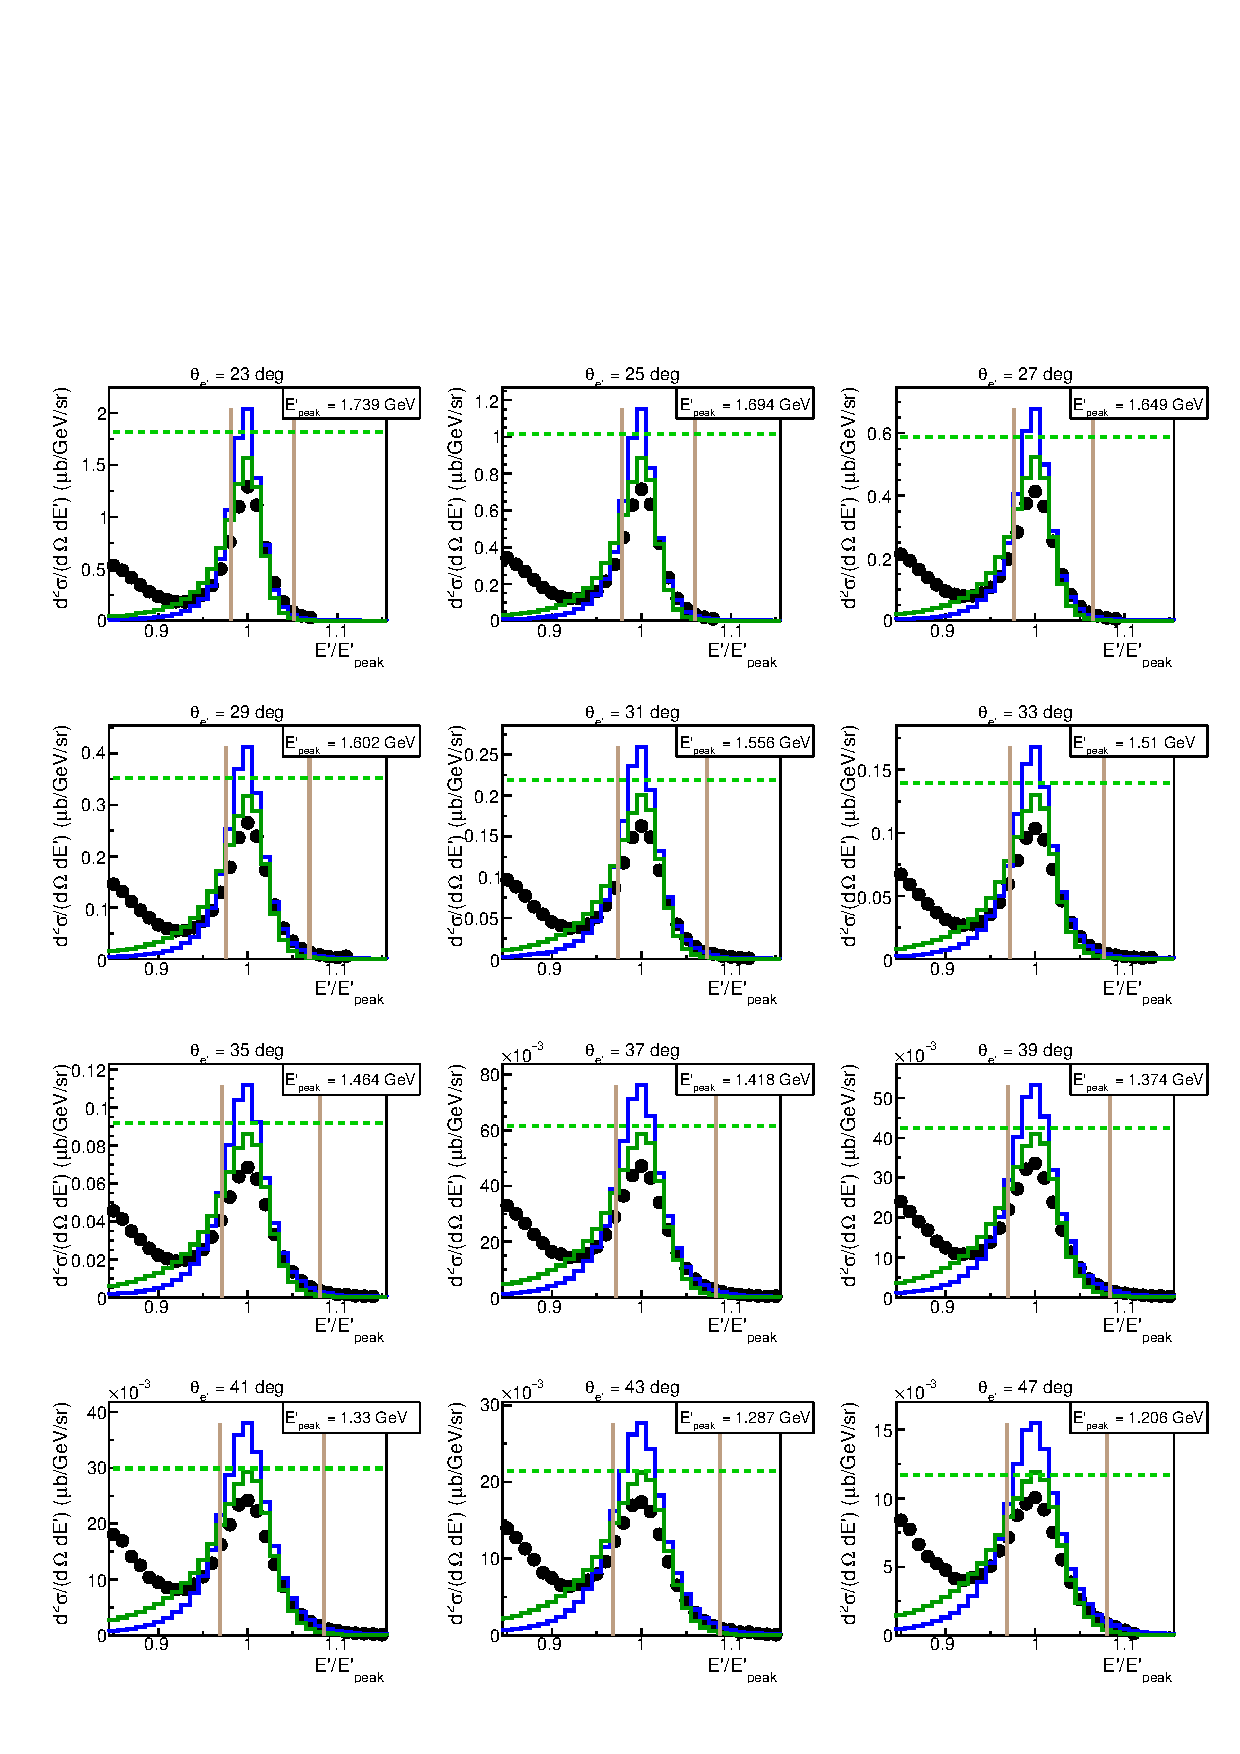
\includegraphics[width=\textwidth]{pictures/normalization/my_xsect_pdf.pdf}
\caption{\small Black symbols correspond to the (radiated) cross section in the region of the quasi-elastic peak extracted from the analyzed dataset according to Eq.~\eqref{eq:my_xsect}. The results of the Bosted parametrization~\cite{Bosted_fit,Bosted:2007xd} are shown by the histograms. The blue histograms correspond to $F^{QE}$ calculated by using the Paris wave function, while the green histograms correspond to $F^{QE}$ given by Eq.~\eqref{eq:fqe_scaling}. The green horizontal lines correspond to Durand's approximation of the peak value given by Eq.~\eqref{eq:durand}. The vertical lines correspond to the left integration limits. } \label{fig:my_QE}
\end{center}
\end{figure}
\begin{table}[htp]
\begin{center}
\caption{\small Ratios of the experimental integrals under the quasi-elastic peak ($\sigma_{exp}$) obtained from the analyzed dataset to those obtained from the Bosted parametrization~\cite{Bosted_fit,Bosted:2007xd} with $F^{QE}$ calculated by using the Paris wave function ($\sigma_{par}^{1}$) and $F^{QE}$ given by Eq.~\eqref{eq:fqe_scaling} ($\sigma_{par}^{2}$). The index $norm$ means that the parametrization histogram was scaled in a way that its maximum was equal to Durand's prediction (see Eq.~\eqref{eq:durand}). The dark-green shade stands for deviations $\leq 5$\%, light-green for 5\%-10\%, light-red for 10\%-20\%, and dark-red for more than 20\%.   \label{tab:quasi_el_tab_my}}

\FloatBarrier

\begin{tabular}{ 
  !{\vrule width 2pt}
  c!{\vrule width 1pt}
  c!{\vrule width 1pt}
  c!{\vrule width 1pt}
  c!{\vrule width 2pt}
  c!{\vrule width 1pt}
  c!{\vrule width 2pt}
  c!{\vrule width 1pt}
  c!{\vrule width 2pt}
 }
\toprule[2pt]
\makecell{$\theta_{e'}$\\ (deg)}  & \makecell{$E'_{peak}$\\ (GeV)} & $R$ &\makecell{$\sigma^{peak}_{Durand}$\\ ($\mu$b)} &$\sigma_{exp}/\sigma_{par}^{1}$ &$\sigma_{exp}/\sigma_{\substack{par,\\norm}}^{1}$ &$\sigma_{exp}/\sigma_{par}^{2}$ &$\sigma_{exp}/\sigma_{\substack{par,\\norm}}^{2}$\\\Xhline{1pt}
23  &1.739  &0.8479  &1.817E0   &\cellcolor{red!20}0.89  &\cellcolor{green!35}1.01  &\cellcolor{green!20}1.07 &\cellcolor{green!20}0.92 \\\Xhline{1pt}
25  &1.694  &0.8467  &1.014E0   &\cellcolor{red!20}0.88  &\cellcolor{green!35}1.00  &\cellcolor{green!35}1.05 &\cellcolor{green!20}0.92 \\\Xhline{1pt} 
27  &1.649  &0.8456  &5.876E-1  &\cellcolor{red!20}0.87  &\cellcolor{green!35}1.00  &\cellcolor{green!35}1.04 &\cellcolor{green!20}0.93 \\\Xhline{1pt} 
29  &1.602  &0.8446  &3.531E-1  &\cellcolor{red!20}0.89  &\cellcolor{green!35}1.04  &\cellcolor{green!20}1.08 &\cellcolor{green!35}0.97 \\\Xhline{1pt} 
31  &1.556  &0.8438  &2.188E-1  &\cellcolor{red!20}0.87  &\cellcolor{green!35}1.03  &\cellcolor{green!20}1.06 &\cellcolor{green!35}0.97 \\\Xhline{1pt} 
33  &1.51   &0.8431  &1.397E-1  &\cellcolor{red!20}0.86  &\cellcolor{green!35}1.03  &\cellcolor{green!35}1.05 &\cellcolor{green!35}0.97 \\\Xhline{1pt} 
35  &1.464  &0.8424  &9.162E-2  &\cellcolor{red!20}0.84  &\cellcolor{green!35}1.03  &\cellcolor{green!35}1.04 &\cellcolor{green!35}0.98 \\\Xhline{1pt} 
37  &1.418  &0.8419  &6.167E-2  &\cellcolor{red!20}0.84  &\cellcolor{green!35}1.04  &\cellcolor{green!35}1.04 &\cellcolor{green!35}0.99 \\\Xhline{1pt} 
39  &1.374  &0.8414  &4.244E-2  &\cellcolor{red!20}0.84  &\cellcolor{green!35}1.05  &\cellcolor{green!35}1.05 &\cellcolor{green!35}1.02 \\\Xhline{1pt} 
41  &1.33   &0.8410  &2.988E-2  &\cellcolor{red!20}0.85  &\cellcolor{green!20}1.08  &\cellcolor{green!20}1.07 &\cellcolor{green!35}1.04 \\\Xhline{1pt}
43  &1.287  &0.8407  &2.147E-2  &\cellcolor{red!20}0.84  &\cellcolor{green!20}1.08  &\cellcolor{green!20}1.06 &\cellcolor{green!35}1.05 \\\Xhline{1pt} 
45  &1.246  &0.8404  &1.571E-2  &\cellcolor{red!20}0.84  &\cellcolor{green!20}1.10  &\cellcolor{green!20}1.07 &\cellcolor{green!20}1.07 \\ \Xhline{1pt}
47  &1.206  &0.8402  &1.171E-2  &\cellcolor{red!20}0.83  &\cellcolor{green!20}1.10  &\cellcolor{green!35}1.05 &\cellcolor{green!20}1.07 \\\bottomrule[2pt]
\end{tabular}
\end{center}
\end{table}\FloatBarrier

\begin{figure}[htp]
\begin{center}
\begin{framed}
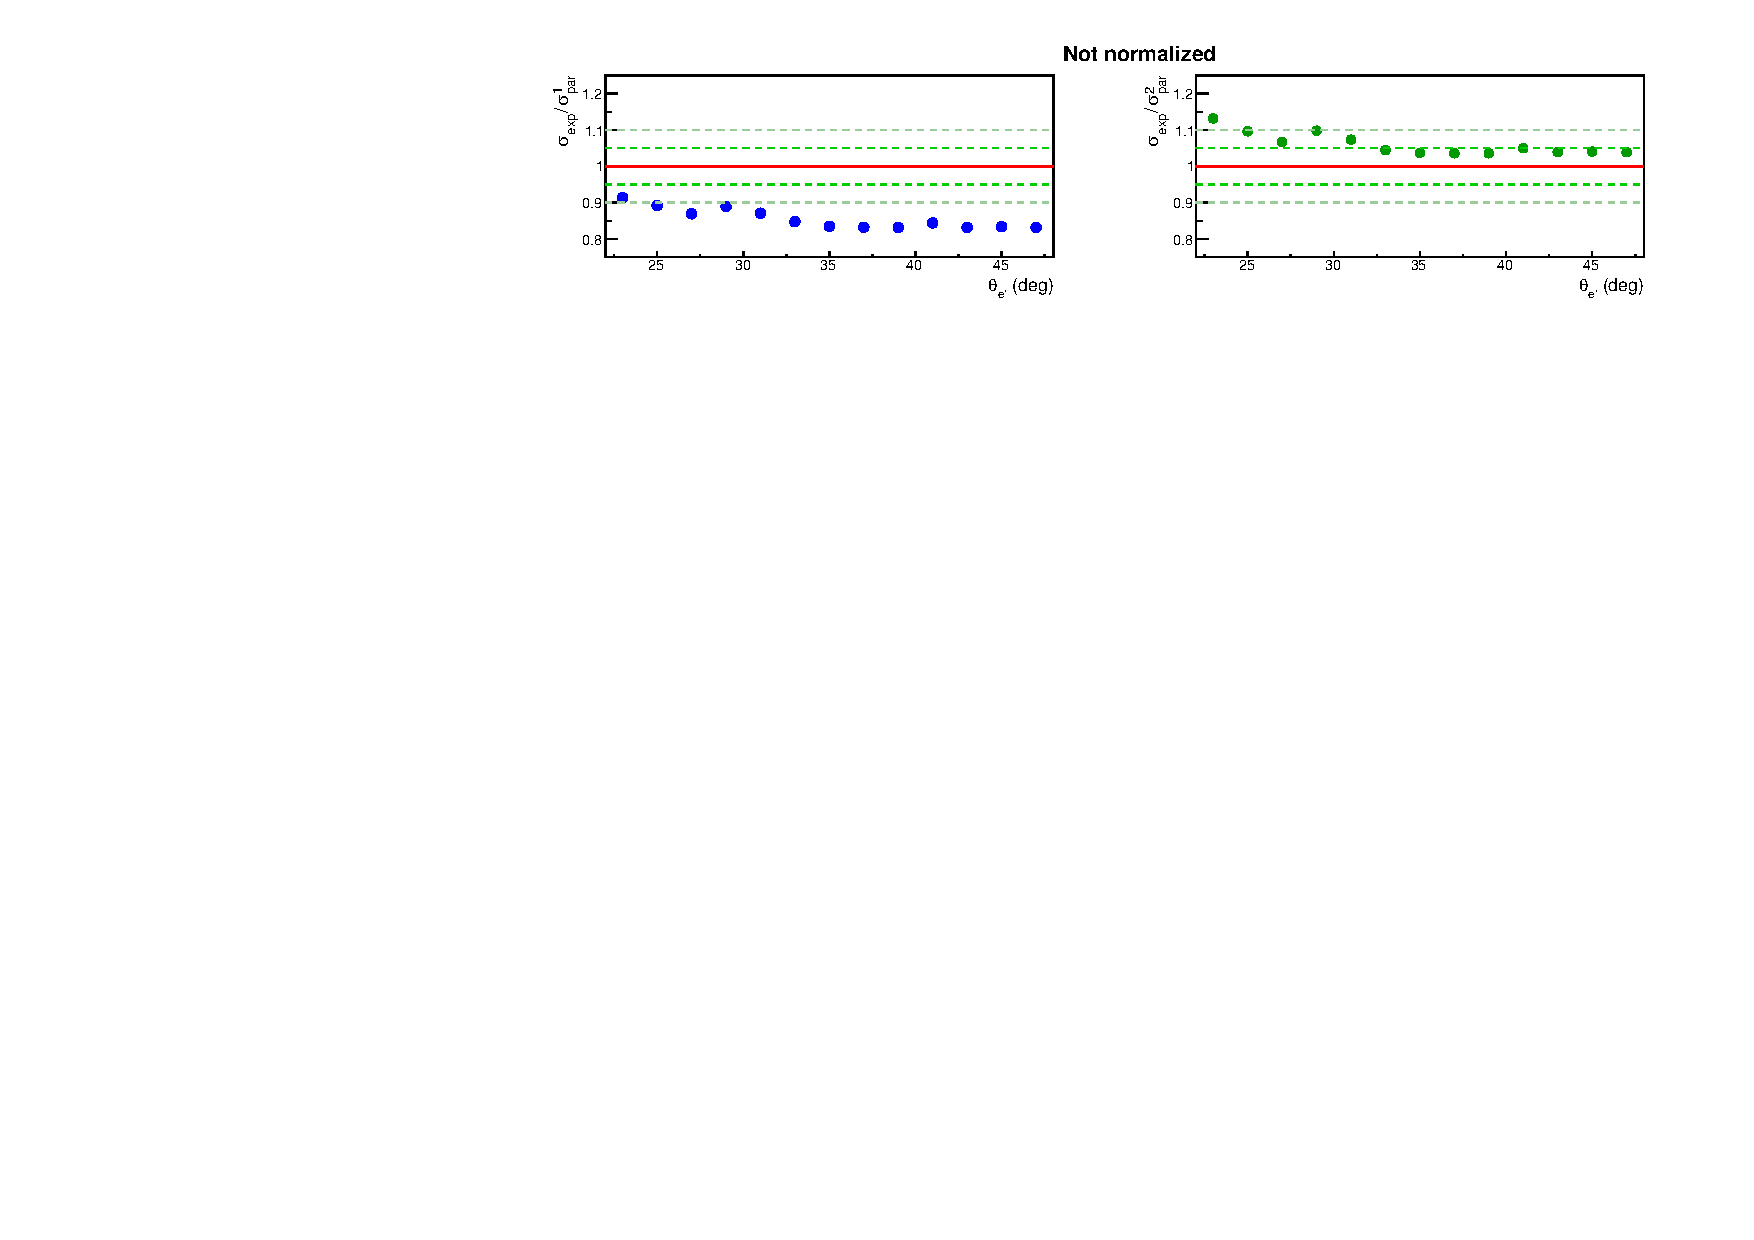
\includegraphics[width=15cm]{pictures/normalization/my_ratio_not_norm.pdf}
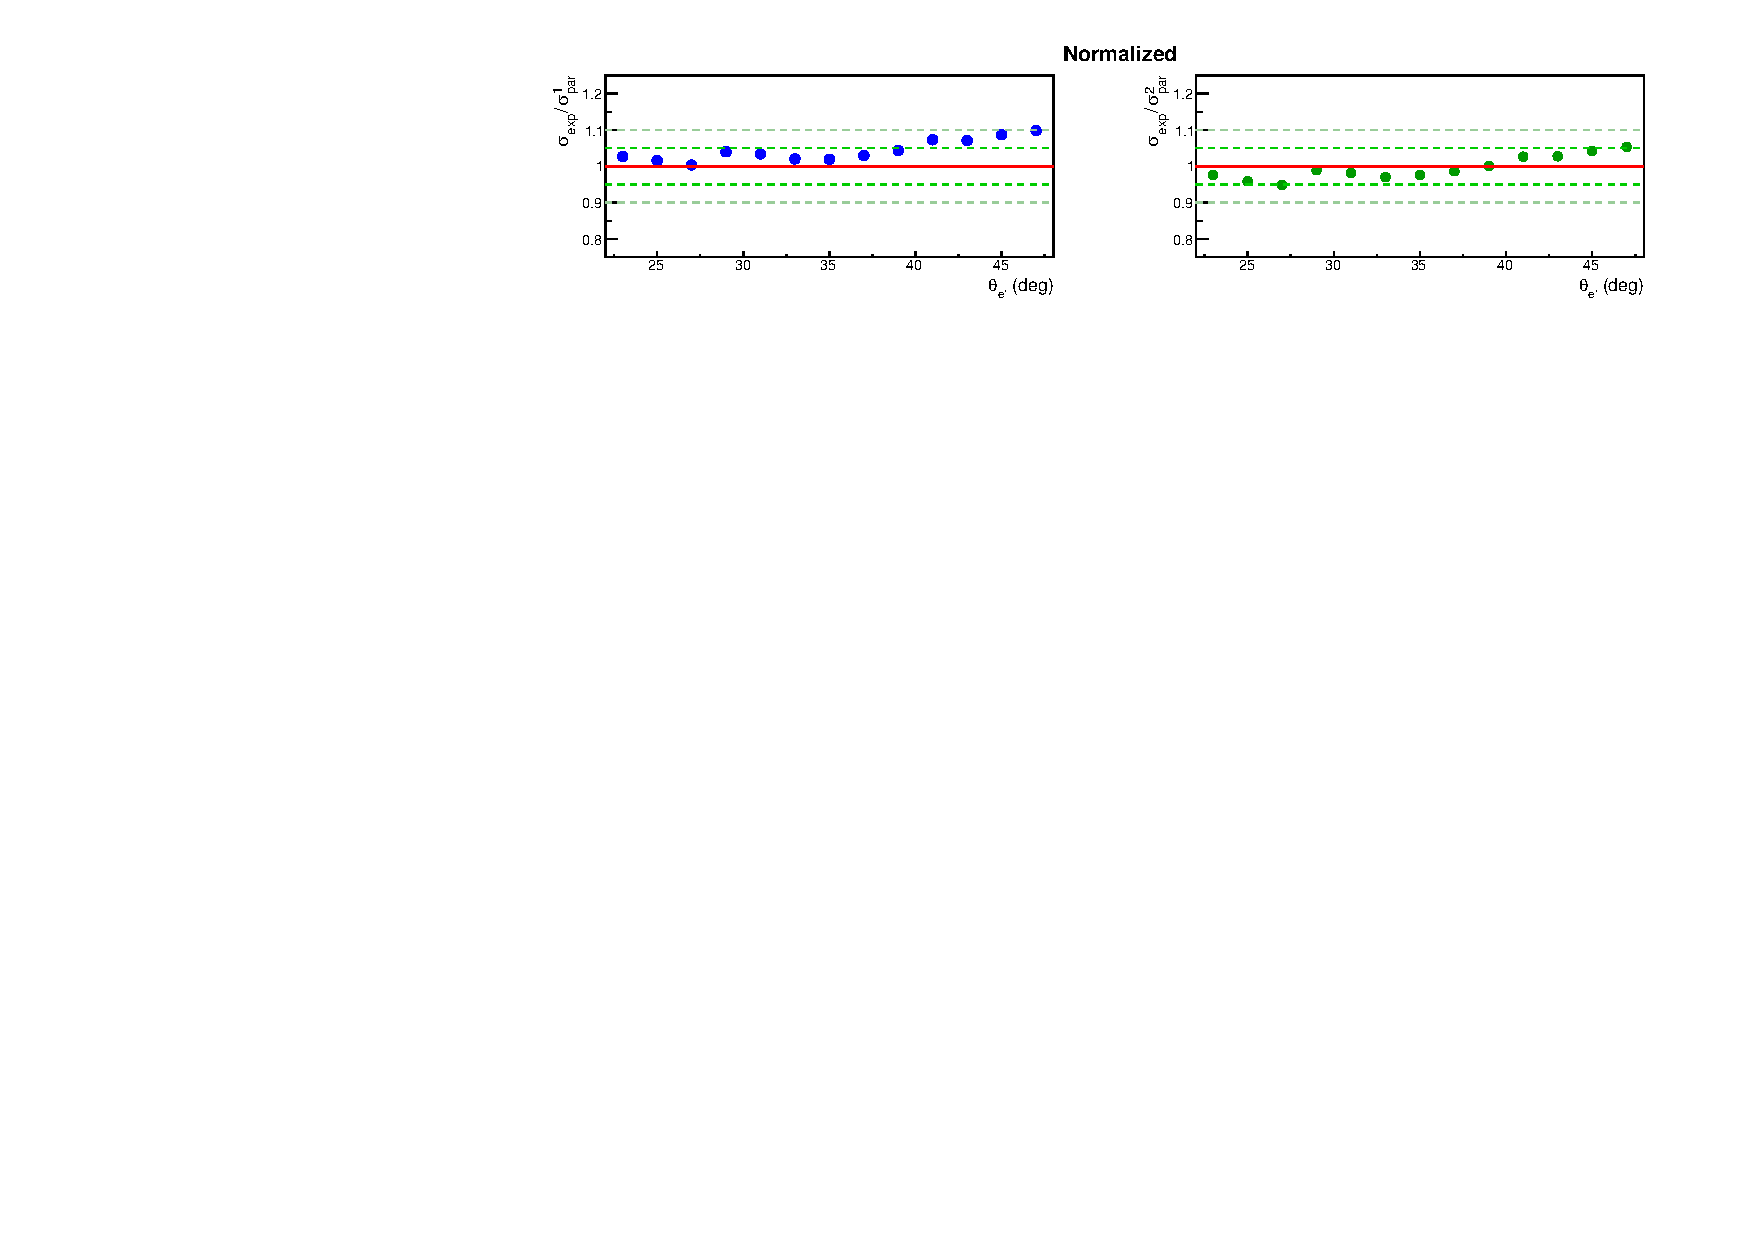
\includegraphics[width=15cm]{pictures/normalization/my_ratio_norm.pdf}
\end{framed}
\caption{\small Ratios of the experimental integral under the quasi-elastic peak to the parametrized one as a function of the angle $\theta_{e'}$. The left side corresponds to the case, when $F^{QE}$ was calculated by using the Paris wave function (blue symbols), while the right side corresponds to $F^{QE}$ calculated according to Eq.~\eqref{eq:fqe_scaling} (green symbols). The top row stands for the unscaled parametrized histograms, while the bottom row corresponds to the case, when they were scaled to the peak value approximated by Durand's formula (see Eq.~\eqref{eq:durand}). The red solid line marks the position of unity. The dark-green dashed lines mark the deviation of 5\%, while the light-green ones show the deviation of 10\%.} \label{fig:my_ratio}
\end{center}
\end{figure}

The cross section calculated according to Eq.~\eqref{eq:my_xsect} is shown by the black symbols in Fig.~\ref{fig:my_QE} (note that it is the radiated cross section). The blue and green histograms in this figure correspond to the Bosted parametrization with  $F^{QE}$ calculated by using the Paris wave function and $F^{QE}$ given by Eq.~\eqref{eq:fqe_scaling}, respectively. The green horizontal lines correspond to Durand's approximation of the peak value given by Eq.~\eqref{eq:durand}.  

Since the experimental cross section is radiated, while the parametrized cross section is not, their visual comparison looses informativeness. To judge more definitely the agreement of the measurement with the parametrization, the corresponding integrals under the quasi-elastic peak were compared. The distributions were integrated from the values shown by the vertical lines in Figs.~\ref{fig:my_QE} (at the position of $0.97\cdot E_{peak}$) up to the right distribution edges. The experimental integrated cross section was then divided by the radiative correction factor ($R$), which was calculated according to the Mo\&Tsai approach~\cite{Mo:1968cg}. The corresponding radiative correction factors as well as the values of $E_{peak}$ are listed in Tab.~\ref{tab:quasi_el_tab_my} for each $\theta_{e'}$ bin. The cross section peak values approximated by Durand's formula (see Eq.~\eqref{eq:durand}) are also given there. The last four columns contain the values of the ratio of the experimental integral under the quasi-elastic peak ($\sigma_{exp}$) to that obtained from the Bosted parametrization with $F^{QE}$ calculated by using the Paris wave function ($\sigma_{par}^{1}$) and $F^{QE}$ given by Eq.~\eqref{eq:fqe_scaling} ($\sigma_{par}^{2}$). The index $norm$ indicates that the parametrization histogram was scaled in a way that its maximum is equal to Durand's approximation. The cells' coloring is the same as for Tab.~\ref{tab:quasi_el_tab}, i.e. the dark-green shade stands for deviations $\leq 5$\%, light-green for 5\%-10\%, light-red for 10\%-20\%,and dark-red shows deviations of more than 20\%.

The ratios of the experimental integrals to the parametrized ones are also shown in Fig.~\ref{fig:my_ratio} as a function of the polar angle of the scattered electron ($\theta_{e'}$). The left side corresponds to the case, when $F^{QE}$ was calculated by using the Paris wave function (blue symbols), while the right side corresponds to $F^{QE}$ being calculated according to Eq.~\eqref{eq:fqe_scaling} (green symbols). The top row stands for the unscaled parametrization histograms, while the bottom row corresponds to the case, when they were scaled to the peak value approximated by Durand's formula. 

As is seen from both Tab.~\ref{tab:quasi_el_tab} and Fig.~\ref{fig:my_ratio}, unscaled parametrization with $F^{QE}$ calculated by using the Paris wave function underestimates the experiment by 10\%-15\%, while with $F^{QE}$ calculated according to Eq.~\eqref{eq:fqe_scaling} is in good agreement with the experiment with a very slight overestimation. Meanwhile, if the parametrization is scaled to Durand's peak value, the ratio stays in the vicinity of unity with a reasonable deviation for both options to calculate $F^{QE}$. This result is consistent with that obtained in the previous subsection for the existing data from Refs.~\cite{Hanson:1973vf,Rock:1991jy,Rock_SLAC}.

Thus, one can conclude that, taking into account some lack of quality of the theoretical description of the quasi-elastic scattering off the deuteron, the measured cross section is in agreement with the available parametrization~\cite{Bosted_fit,Bosted:2007xd}. This, in turn, indicates that in this particular analysis both the electron selection and overall normalization are under control.


%\begin{equation}
%\sigma_{exp} (\theta_{e'}) = \frac{1}{R}\cdot \!\!\! \!\!\!\int \limits_{0.97E_{peak}}^{1.2E_{peak}} \frac{d\sigma_{exp}}{d\Omega dE'}\cdot dE' ,
%\end{equation}



\counterwithin{equation}{section}


